\chapter{Resultados \emph{software}}
\label{ch:resultados_sw}

% %* Comprobar
% En el siguiente capitulo se van a comentar los diversos resultados obtenidos en el presente TFG, tanto los relacionados con la FPGA (\emph{hardware} usado, simulaciones y sintetizado final), como con el \emph{software} de control. Se incluyen además, varias imágenes que complementen las explicaciones del mismo.

%!
Aun teniendo más importancia la parte \emph{hardware} comentada en el capitulo~\ref{ch:resultados_hw}, el sistema no sería funcional sin una aplicación que utilice los recursos creados para recibir y almacenar la captura. Por eso, se ha creado una aplicación que incluye además varias opciones de configuración.

%! Revisar
\section{Aplicaciones de apoyo}
A medida que se ha ido desarrollando la parte \emph{hardware}, se han creado varias utilidades en lenguaje \emph{Python}, con las que realizar cálculos de forma rápida o con las que comprobar el funcionamiento de ciertas partes del sistema. Dichas aplicaciones se encuentran en el directorio \emph{.\textbackslash ICEstick\textbackslash USB3300\_sniffer\textbackslash tools\textbackslash} del repositorio. \\
Hay que destacar las siguientes:
\begin{enumerate}
    %* Comprobar
    \item \textbf{Utilidad de divisiones del reloj (\emph{get\_divider.py}).} \\
    Utilidad con la que poder realizar de forma rápida varios cálculos relacionados con los relojes de entrada. Por ejemplo, obtener los valores óptimos con los que dividir un reloj para generar unos baudios deseados. En el listado \ref{src:utilidad_divisiones_reloj_out} se plasma un ejemplo de uso.
    \begin{lstlisting}[
        caption={Ejemplo de la utilidad de divisiones de reloj.},
        label=src:utilidad_divisiones_reloj_out]
$ ./get_divider.py
  Usage: ./get_divider.py [option] arg1 arg2
  Options: 
      -o: Print the optimal counter value for a given clock (arg1) and Serial baudrate (arg2). [Default]
      -b: Print the minimal divider value for a given clock (arg1) and Serial baudrate (arg2).
      -d: Print the minimal divider value for a given clock (arg1) and time (arg2).
      -t: Print the time (and serial baudrate) for a given clock (arg1) and divider (arg2).
      -a: Print, for a given clock (arg1), all the possible periods that can be generated between 0 and arg2.
      -c: Print the clock for a given time (arg1) and divider (arg2).
$ ./get_divider.py -o 12000000 115200
  Optimal counter value: 105
$ ./get_divider.py -b 12000000 9600
  Recomended divider (with 18% error): 10 [8.533333333333334e-05s]
  10 [8.533333333333334e-05s] - [0.00010416666666666667s] - 11 [0.00017066666666666668s]          
    \end{lstlisting}
    
    %! Revisar
    \item \textbf{Utilidad de generación de baudios (\emph{gen\_bauds.py}).} \\
    Pequeña aplicación que, para los $baudios$ más comunes, genere varias definiciones de \emph{Verilog}, a usar por el módulo encargado de generar el reloj de baudios. En el listado \ref{src:utilidad_baudios_out} se muestra un ejemplo de la salida de la aplicación ante un reloj de $60MHz$.
%     \\ \noWord[Borrar listado??? La verdad, es algo inutil ponerlo]
    \begin{lstlisting}[
        caption={Ejemplo de la utilidad de generación de baudios ante \emph{60 MHz} de entrada.},
        label=src:utilidad_baudios_out]
$ ./gen_bauds.py
  `define B921600 66
  `define B460800 131
  `define B256000 235
  `define B230400 261
  `define B153600 391
  `define B128000 469
  `define B115200 521
  `define B57600  1042
  `define B56000  1072
  `define B38400  1563
  `define B28800  2084
  `define B19200  3125
  `define B14400  4167
  `define B9600   6250
  `define B4800   12500
  `define B2400   25000
  `define B1200   50000
  `define B600    100000
  `define B300    200000
  `define B110    545455
    \end{lstlisting}
    
    %! Revisar
    \item \textbf{Utilidad de control serie (\emph{serial\_control.py}).} \\
    Aplicación, que usando una librería encargada de controlar puertos serie, realiza varias comprobaciones del protocolo creado. Esta se puede configurar para abrir el puerto serie a cualquier velocidad, y poder enviar comandos de prueba.
\end{enumerate}

%!
\section{Información de la aplicación}
Tal como se ha comentado al principio de este capítulo, aun teniendo mayor carga la parte \emph{hardware}, es esencial implementar una aplicación que se comunique con la FPGA y permita su funcionamiento.

Para ello, utilizando lenguaje C, se ha creado una aplicación que dando opciones de control con una simple interfaz, es capaz de enviar comandos o recibir datos USB, y a su vez, es capaz de almacenarlos para su posterior estudio.

La aplicación se ha dividido de la siguiente manera:
\begin{enumerate}
    %* Comprobar
    \item \textbf{Hilo encargado de controlar las entradas de usuario.} \\
    Tanto la configuración a usar para conectarse a la \emph{FPGA} (puerto serie y su velocidad), como los comandos a enviar, son introducidos al programa por medio de un simple menú basado en texto desde la terminal. Este permite:
    \begin{itemize}
        \item Configurar el puerto serie (puerto a usar y velocidad en baudios).
        \item Abrir/cerrar el puerto seleccionado.
        \item Realizar una operación de lectura de registro.
        \item Realizar una operación de escritura de registro.
        \item Activar/desactivar el envío de datos USB al PC.
    \end{itemize}

    En la figura~\ref{fig:matriz-app-menu} se muestra dicho menú, y a su vez, se ejemplifica un proceso de escritura y posterior lectura del registro con dirección \emph{0x16} (registro que según la hoja de características del integrado USB3300\cite{microchip:usb3300} es de libre utilización).

    \begin{figure}[htbp]
        \centering
        \subfigure[Operación de escritura]{
            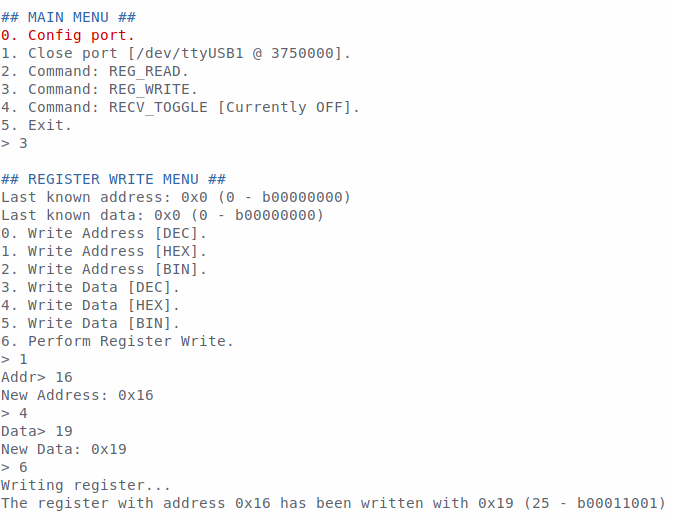
\includegraphics[width=100mm]{menu_app/escrituraB.png}
            \label{fig:matriz-hw-resto:cables}
        }
        \subfigure[Operación de lectura]{
            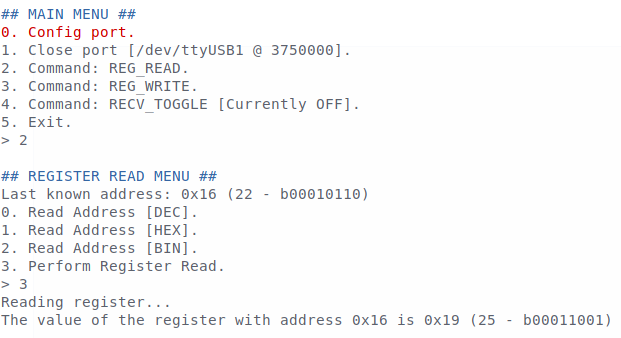
\includegraphics[width=100mm]{menu_app/lecturaB.png}
            \label{fig:matriz-hw-resto:botones}
        } \\
        \caption{Ejemplo de escritura de registro y su posterior lectura usando el menú de la aplicación} 
        \label{fig:matriz-app-menu}
    \end{figure}
    
    %* Comprobar
    \item \textbf{Hilo encargado de gestionar la comunicación con la \emph{FPGA}, así como almacenar la trama capturada.} \\
    Este hilo maneja toda la comunicación serie entre la FPGA, ya sea para enviar comandos, o para recibir los datos USB capturados. Al finalizar el proceso de recepción de datos, es este hilo el encargado también de guardar la captura en un archivo para su posterior análisis.
\end{enumerate}


%!
\section{Información del archivo generado}
Se ha elegido almacenar la información capturada en un archivo formato JSON\footnote{Formato de texto, que permite almacenar información de forma estructurada.}. Este archivo, posee una estructura fi

\begin{figure}[!hbtp]
    \centering
    \begin{minipage}{5cm}
        \dirtree{%
            .1 date.
            .1 USB\_data.
            .2 captura[0].
            .3 TxCMD.
            .3 DataLen.
            .3 data.
            .4 data[0].
            .4 \ldots.
            .4 data[DataLen-1].
            .2 \ldots.
            .2 captura[n].
        }
    \end{minipage}
    \caption{Estructura del archivo JSON donde se almacena la captura}
    \label{fig:tree-json}
\end{figure}

%!
\section{Conversión de JSON a PCAP}
Para poder analizar la captura en la aplicación de analisis \emph{Wireshark}, se ha creado otra utilidad, que a partir del archivo JSON generado anteriormente lo transforma a PCAP.
Su uso 

\begin{lstlisting}[
    caption={Ejemplo de la utilidad de generación de baudios ante \emph{60 MHz} de entrada.},
    label=src:utilidad_baudios_out]
$ ./gen_bauds.py
`define B921600 66
`define B460800 131
`define B256000 235
`define B230400 261
`define B153600 391
`define B128000 469
`define B115200 521
`define B57600  1042
`define B56000  1072
`define B38400  1563
`define B28800  2084
`define B19200  3125
`define B14400  4167
`define B9600   6250
`define B4800   12500
`define B2400   25000
`define B1200   50000
`define B600    100000
`define B300    200000
`define B110    545455
\end{lstlisting}




% \chapter{Resultados}
% \label{ch:resultados-plantilla}

% Escribe en este capítulo los resultados del proyecto.  Este capítulo debería explicar los resultados de forma global, no los resultados de cada iteración.  Probablemente será el capítulo con más tablas y gráficas.  Revisa las secciones~\ref{sec:figuras} y~\ref{sec:tablas} para aprender cómo se escriben en \LaTeX{}.